\documentclass[a4paper, 12pt, oneside]{report}
\usepackage[margin=1in]{geometry}
\usepackage[table]{xcolor}
\usepackage{amsmath}
\usepackage{amssymb}
\usepackage{graphicx}
\usepackage[toc,page]{appendix}
\usepackage[numbers]{natbib}
\usepackage{chemformula}
\usepackage{fancyhdr}
\usepackage{lipsum}
\usepackage{float}
\usepackage{booktabs}
\PassOptionsToPackage{hyphens}{url}\usepackage[hidelinks]{hyperref}
\usepackage{multirow}
\usepackage{caption}
\usepackage{subcaption}
\usepackage{array}
\usepackage{setspace}
\usepackage{titletoc}
\usepackage{enumerate}
\usepackage{mathptmx}
\usepackage{fontspec}
\usepackage{listings}
\usepackage{xcolor}
\usepackage{natbib}
\usepackage{fancyhdr}
\usepackage{hyperref}
\lstset{
    language=Python,
    basicstyle=\ttfamily\small,   
    keywordstyle=\color{blue},     
    commentstyle=\color{green},    
    stringstyle=\color{red},       
    showstringspaces=false,        
    numberstyle=\tiny\color{gray}, 
    stepnumber=1,                  
    numbersep=5pt,                 
    backgroundcolor=\color{white}, 
    frame=single,                  
    rulecolor=\color{black},       
    breaklines=true,               
    breakatwhitespace=true,        
    tabsize=4,                     
    captionpos=b,                  
    escapeinside={\%*}{*)}         
}
\setmainfont{Times New Roman}

\renewcommand{\thechapter}{\Roman{chapter}}
\usepackage[french]{babel}

\setlength{\headheight}{15pt}
\setstretch{1.20}

\begin{document}

\begin{titlepage}
\newgeometry{top=0.5in,left=0.5in,right=0.5in}

\includegraphics[width = 0.16 \textwidth]{fig/Image2.png} \hfill
\begin{minipage}[b][3.26 \baselineskip][t]{20 em}
\centering
Université Ibn Zohr  \\
Faculté des sciences \\
Centre d'excellence IT\\
\end{minipage} \hfill  

\includegraphics[width = 52mm]{fig/logo1.png}

\hrule

\vspace{3 cm}
\begin{center}
\LARGE{\textbf{Master d'Excellence Ingenierie Logicielle}}
\end{center}
\vspace{1 cm}
\begin{center}
\LARGE{\textbf{Rapport}}
\end{center}

\vspace{1.3 cm}
\hrule
\begin{center}
\huge{\textbf{Projet de Data Mining et d'Analyse des Données : Exploration et Analyse des Prix et des Promotions des Produits Électroménagers}}
\end{center}
\hrule

\vspace{1.5 cm}
\begin{center}
\LARGE{\textbf{Réalisé par :}}
\end{center}

\vspace{0.1 cm}
\begin{center}
\Large{Youssef BOUALI}
\end{center}

\vspace{1.9 cm}
\hrule
\begin{center}
\Large{\textbf{Encadré par :} \ \ \  
Prof. Rajae BENSOLTANE} 
\end{center}

	\hrule
	\vspace{ 1 cm}
	\begin{center}
	\Large{\textbf{Année universitaire :} 2024/2025}
	\end{center}
\end{titlepage}

%\pagenumbering{Roman} 
%\pagestyle{styletoc}

\begin{abstract}
Ce projet porte sur l'analyse des variations des prix et des promotions des produits électroménagers à travers plusieurs plateformes de commerce en ligne. L'objectif est de comparer les stratégies tarifaires et promotionnelles utilisées par les principales plateformes e-commerce dans le secteur de l'électroménager. En utilisant des techniques de \textit{web scraping}, les données ont été collectées sur des sites tels que BestBuy, LG, et Samsung. Ces informations ont été nettoyées, préparées et analysées pour identifier les tendances de prix, les périodes de promotions, ainsi que les effets de ces dernières sur les stratégies de prix. Les résultats obtenus sont présentés sous forme de graphiques permettant de visualiser les écarts de prix entre les plateformes, la fréquence des promotions, ainsi que l'évolution temporelle des prix. Cette analyse fournit des informations précieuses pour comprendre les pratiques tarifaires dans le secteur des produits électroménagers et pourrait aider les consommateurs à faire des choix plus éclairés lors de leurs achats en ligne.
\end{abstract}

%\thispagestyle{empty}
\renewcommand*{\contentsname}{Table des matières}
\begin{doublespace}
%\clearpage
\tableofcontents
%\cleardoublepage
\end{doublespace}
\cleardoublepage

\phantomsection
\addcontentsline{toc}{chapter}{Liste des figures}
\renewcommand*{\listfigurename}{Liste des figures}
%\clearpage
\listoffigures

%\pagenumbering{arabic}

%\pagestyle{stylenor}

\chapter{Introduction Générale}
L'évolution des prix et des promotions dans le secteur des électroménagers est influencée par des facteurs multiples tels que la saisonnalité, les événements de vente et la concurrence. Ce projet se propose d’analyser ces éléments à partir des données collectées sur plusieurs plateformes de commerce en ligne populaires. L'objectif est d’identifier les meilleures offres et de mieux comprendre les stratégies tarifaires dans ce domaine spécifique.

\bigskip

Ce projet vise à étudier les variations des prix et des promotions pour des produits électroménagers similaires ou identiques sur différentes plateformes de vente en ligne. En se concentrant sur cette catégorie de produits, l'analyse cherchera à comprendre les tendances tarifaires et les stratégies promotionnelles adoptées par les grandes plateformes e-commerce dans le secteur des électroménagers.

\bigskip

À travers cette étude, il sera possible d’identifier les meilleures offres disponibles en ligne et d’approfondir la compréhension des dynamiques tarifaires, tout en offrant des recommandations utiles aux consommateurs pour prendre des décisions d’achat éclairées. Les résultats obtenus pourraient également fournir des pistes pour améliorer leurs stratégies de pricing et de promotions, en fonction des tendances observées sur les différentes plateformes.


\chapter{Problématique}
Dans le secteur de l’électroménager, les consommateurs sont confrontés à une grande variété de prix et de promotions qui diffèrent selon les plateformes de commerce en ligne. Ces différences peuvent rendre difficile la prise de décision lors de l'achat d'un produit. Il devient ainsi essentiel de comprendre comment les plateformes e-commerce déterminent leurs stratégies tarifaires et leurs promotions pour les produits électroménagers.

\begin{quote}
    \textit{L'objectif est d'analyser ces dynamiques afin de fournir aux consommateurs des informations utiles et à jour, facilitant ainsi leurs choix, et offrant aux entreprises des pistes d'amélioration pour leurs stratégies commerciales.}
\end{quote}


\chapter{Méthodologie}

\section{Objectif}
L'objectif principal du projet est de :
\begin{itemize}
    \item Analyser les prix des produits électroménagers identiques ou similaires sur différentes plateformes de commerce en ligne.
    \item Identifier les périodes de promotions et les stratégies tarifaires spécifiques dans le secteur de l’électroménager.
    \item Comparer les prix moyens et les offres promotionnelles des produits électroménagers à travers plusieurs plateformes populaires.
\end{itemize}


\section{Choix de catégorie des produits}
Les produits à analyser seront sélectionnés parmi les catégories suivantes :

\begin{itemize}
    \item \textbf{Produits électroménagers}, en raison de leur forte demande et de la diversité des sous-catégories disponibles.
\end{itemize}

Un échantillon représentatif de ces produits sera choisi afin de garantir une analyse approfondie et pertinente.

\section{Conformité aux conditions d'utilisation}
Pour éviter tout conflit juridique, le scraping sera réalisé dans le strict respect des conditions d’utilisation de chaque plateforme. Des précautions seront mises en place pour réduire les risques de blocage, notamment par l’ajout de délais entre les requêtes et le respect des directives dans les fichier \textit{robots.txt}, les politiques de confidentialité ainsi que les termes et conditions des sites concernés.
De plus, les données collectées seront utilisées exclusivement à des fins éducatives et ne seront en aucun cas exploitées à des fins commerciales ou autres.


\section{Collecte des données}
Pour cette analyse, les données seront collectées de plusieurs plateformes populaires qui vendent des produits électroménagers, telles que applianceworldonline.com, sharpusa.com, costo.com, bestbuy.com, lg.com, samsung.com, sears.com et us-appliance.com. En raison de la disponibilité limitée des APIs ou de l'existence d'APIs payantes, la collecte des données sera effectuée principalement à travers une autre méthode :

\begin{itemize}
    \item \textbf{Web scraping} : Comme les plateformes e-commerce ne fournissent pas d'APIs gratuites ou disponibles pour l'extraction des données, le scraping des pages des produits sera utilisé pour extraire directement les informations nécessaires. Cette méthode permettra de récupérer des données telles que les prix, les promotions et les spécifications des produits. Le scraping sera effectué en conformité avec les lois sur la protection des données et les conditions d'utilisation des sites web. Pour améliorer la rapidité et l'efficacité, plusieurs techniques ont été utilisées :
    \begin{itemize}
        \item \textbf{Selenium} : \textit{Selenium} est un outil d'automatisation de navigateurs web qui permet d'interagir avec des pages web de manière programmée. Il est couramment utilisé pour automatiser des tests sur des applications web ou pour effectuer du web scraping, notamment pour les sites dynamiques.\cite{SeleniumSource}. Utiliser Selenium avec des paramètres spécifiques pour désactiver le chargement des images et la gestion des notifications permet d'accélérer le processus de collecte des données.
    
    \item \textbf{RapidFuzz} : \textit{RapidFuzz} est une bibliothèque Python permettant de réaliser des correspondances rapides de chaînes de caractères pour une correspondance approximative. Elle est plus rapide que FuzzyWuzzy et est couramment utilisée dans des processus de scraping où des comparaisons de texte sont nécessaires pour déterminer des correspondances.\cite{RapidfuzzSource}. Cette bibliothèque a été utilisée comme alternative à FuzzyWuzzy pour une correspondance rapide des chaînes de caractères, ce qui améliore la performance du processus de scraping.
    
    \item \textbf{Threads (Utilisation des threads)} : Un \textit{thread} est une unité d'exécution d'un processus. L'implémentation des threads permet de paralléliser les tâches, ce qui réduit le temps nécessaire pour exécuter plusieurs tâches simultanément. Des threads ont été implémentés pour paralléliser le processus de scraping, réduisant ainsi le temps de collecte des informations sur les produits.
    
    \item \textbf{Conversion des devises} : La \textit{conversion des devises} consiste à ajuster les prix des produits ou services d'une monnaie à une autre (par exemple, de l'euro au dollar américain). Une fonctionnalité a été intégrée pour convertir les prix des produits en devises locales (par exemple, de l'euro au dollar américain), afin d’uniformiser les données pour les comparaisons.
    
    \item \textbf{Cron job sur Ubuntu Server} : Un \textit{cron job} est une tâche planifiée qui est exécutée automatiquement à des intervalles réguliers sur un serveur Linux, comme Ubuntu. Il est utilisé pour automatiser des processus tels que le scraping à des horaires précis, garantissant que les données extraites sont mises à jour régulièrement.\cite{CronjobSource}. Pour automatiser le processus de scraping à intervalles réguliers, un cron job a été configuré sur un serveur Ubuntu. Ce cron job exécute le script de scraping à une heure précise chaque jour, garantissant ainsi que les données extraites sont régulièrement mises à jour.
        \begin{itemize}

            \item \texttt{crontab -e} : Ouvre l'éditeur pour ajouter ou modifier les tâches cron.
            \item Exemple de configuration : 
            \begin{verbatim} {Minute} {Heure} * * * /usr/bin/python3 /scraping/projetElectromenagers.py
            \end{verbatim}
            Cette ligne exécute le script \texttt{projetElectromenagers.py} tous les jours.
        \end{itemize}
    \end{itemize}
\end{itemize}

Le web scraping offrira une flexibilité pour collecter des informations actualisées à partir des différentes plateformes de manière efficace, tout en respectant les politiques de chaque site.

\section{Nettoyage et préparation des données}
Une fois les données collectées, elles seront nettoyées et préparées pour l’analyse. Cela comprendra :
\begin{itemize}
    \item \textbf{Uniformisation des noms de produits} : Les produits identiques peuvent être référencés différemment d’une plateforme à l’autre, il est donc nécessaire d’harmoniser les noms des produits pour assurer une comparaison précise. De plus, les couleurs et autres éléments non pertinents dans les noms des produits seront supprimés pour garantir une normalisation efficace des informations.
    \item \textbf{Suppression des caractères inutiles et normalisation} : Les données peuvent contenir des caractères spéciaux ou des espaces excessifs. Ces éléments seront supprimés. La conversion des majuscules en minuscules sera également effectuée pour garantir la cohérence des informations dans l'ensemble des données.
    \item \textbf{Suppression des produits dupliqués} : Dans une même plateforme et pour une date de scraping donnée, les produits qui apparaissent plusieurs fois seront éliminés pour éviter les doublons et garantir que l'analyse repose sur des données uniques et fiables.
\end{itemize}

\begin{figure}
    \centering
    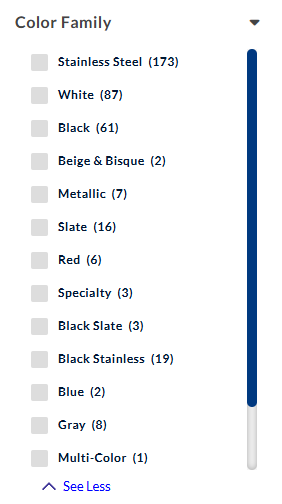
\includegraphics[width=0.3\linewidth]{fig/7.png}
    \caption{Exemple des variations inutiles}
    \label{fig:variations}
\end{figure}
\begin{figure}
    \centering
    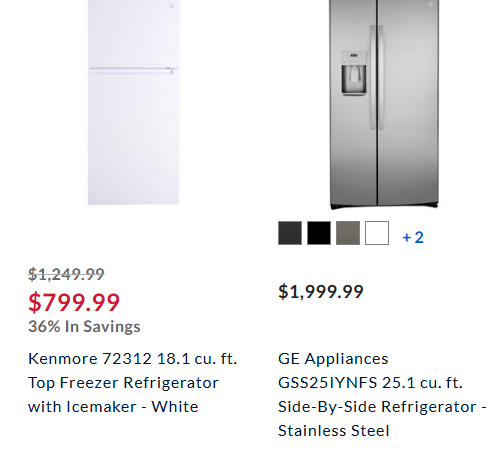
\includegraphics[width=0.3\linewidth]{fig/8.png}
    \caption{Exemple des variations inutiles dans le titre}
    \label{fig:variations2}
\end{figure}


\chapter{Analyse des données}
\section{Comparaison des prix des produits électroménagers}
L'analyse principale du projet sera centrée sur la comparaison des prix des produits électroménagers entre différentes plateformes. Nous allons :
\begin{itemize}
    \item Comparaison le prix pour un produit sur chaque plateforme.
    \item Identifier les sites ayant des écarts de prix significatifs.
\end{itemize}

\section{Identification des promotions spécifiques aux produits électroménagers}
Une attention particulière sera accordée à l'identification des promotions pour les produits électroménagers. Les étapes suivantes seront réalisées :
\begin{itemize}
    \item Identification des promotions spécifiques à cette catégorie de produits (réductions de prix, offres spéciales).
    \item Analyse des périodes de promotions, notamment pendant les événements ou les promotions de début d'année.
    \item Comparaison des effets des promotions sur les prix avant, pendant, et après les événements de promotion.
\end{itemize}

L'analyse des promotions visera à identifier les meilleures stratégies tarifaires adoptées par les plateformes pour attirer les consommateurs tout en maintenant leur rentabilité.

\chapter{Visualisation des résultats}
\section{Visualisation des données}
Les résultats de l’analyse seront présentés sous forme de graphiques.
\begin{itemize}
    \item Des \textbf{histogrammes} pour observer la répartition des prix des produits électroménagers.
    \item Des \textbf{diagrammes en barres} pour comparer les prix et les promotions des produits à une date donnée..
\end{itemize}

\section{Visualisation et résultats}
\subsection{Écarts de prix des produits entre plateformes}
L'analyse des données extraites de la première graph montre les variations de prix pour le plus fréquent \textbf{Price Variations for lg 2.1 cu. ft. wi-fi enabled over-the-range microwave oven with easyclean Across Websites} sur différents sites web. Les écarts de prix mettent en évidence une fluctuation notable, bien que les valeurs exactes ne soient pas entièrement lisibles. Il est à noter que \textbf{Costco.com} apparaît comme la plateforme la plus chère pour ce produit. Ce type de graphique permet d'identifier les tendances de prix et d'aider à la prise de décision pour l'achat de ce produit.

\begin{figure}[H]
    \centering
    
\includegraphics[width=1\textwidth]{fig/output_13_1.png}
    \caption{Écarts de prix entre plateformes}
    \label{fig:output1}
\end{figure}

\subsection{Fréquence des promotions par catégorie}
L'analyse des données extraites de la deuxième graph révèle une distribution des promotions par catégorie et type. Quelques types de promotions notables incluent :
\begin{itemize}
    \item \textit{Appliances : Flash Sale!} (Une vente à durée limitée, où des produits sont proposés à des prix réduits pendant une période restreinte.),
    \item \textit{refrigerators : Jaunary Savings} (Des promotions ou des réductions spéciales offertes en janvier, souvent utilisées pour encourager les achats après les fêtes de fin d'année).
\end{itemize}

Un histogramme illustre les fréquences des promotions, permettant d'identifier les catégories avec les promotions les plus fréquentes.

\begin{figure}[H]
    \centering
    
\includegraphics[width=1\textwidth]{fig/output_13_3.png}
    \caption{Fréquence des promotions par catégorie.}
    \label{fig:output3}
\end{figure}

\subsection{Analyse temporelle des prix et promotions}Écarts de prix moyens entre plateformes
L'évolution des promotions et des prix dans le temps pour des produits les plus fréquents peut être observée à travers les graphiques obtenus. Bien que les données extraites ici soient limitées, une analyse détaillée des tendances temporelles permettrait de mieux comprendre les stratégies marketing des plateformes de vente.

\begin{figure}[H]
    \centering
    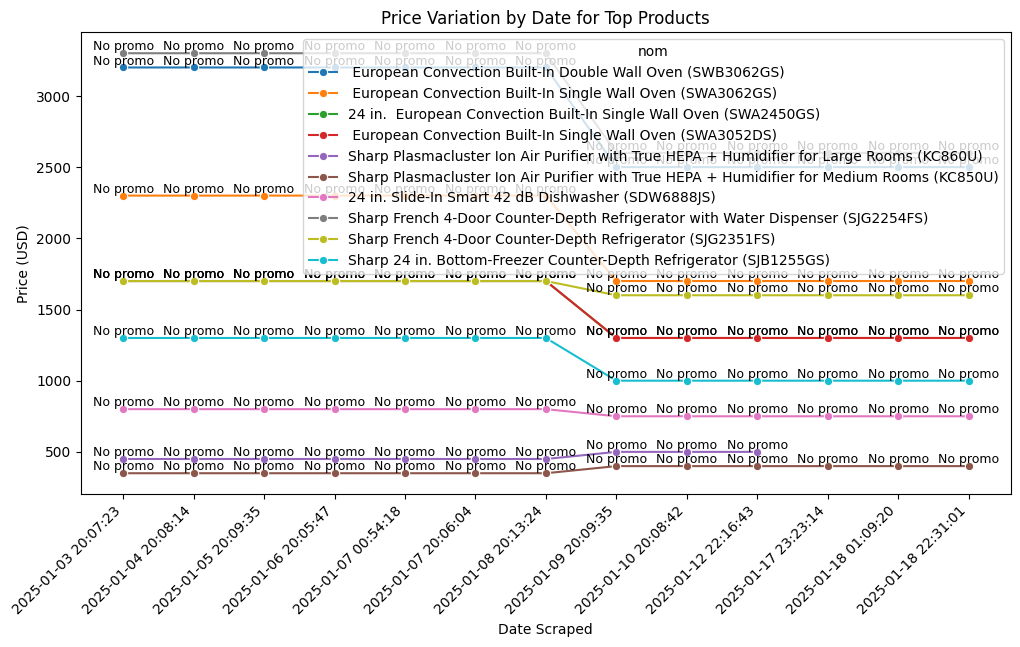
\includegraphics[width=1\textwidth]{fig/output_13_5.png}
    \caption{Analyse temporelle des prix et promotions.}
    \label{fig:output5}
\end{figure}

\subsection{Écarts de prix moyens entre plateformes}
Cette section analyse les différences de prix moyens entre les différentes plateformes de vente. Le graphique ci-dessous illustre les écarts moyens de prix observés pour les plateformes.

\begin{figure}[H]
    \centering
    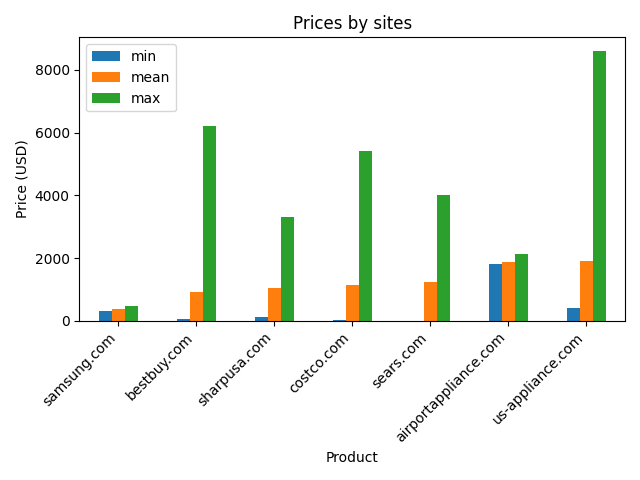
\includegraphics[width=1\textwidth]{fig/output_13_7.png}
    \caption{Écarts de prix entre plateformes.}
    \label{fig:output7}
\end{figure}

Ces visualisations permettront de rendre l’analyse plus compréhensible et de tirer des conclusions sur les stratégies tarifaires dans le secteur de l’électroménager.
Il est à noter que \textbf{Samsung.com} propose les prix les plus bas, tandis \textbf{que US-Appliance.com} affiche les tarifs les plus élevés.


\chapter{Développement de l’API}
\section{Service API}
Une API développée pour permettre aux utilisateurs d'utiliser des fonctionnalités d'analyse. Cette API pourra offrir des fonctionnalités comme :
\begin{itemize}
    \item \textbf{Récupérer le prix le plus bas d’un produit électroménager} : L'utilisateur peut entrer un nom de produit et obtenir les prix les plus bas sur différentes plateformes.
    \item \textbf{Lister les promotions actuelles} : L'API pourra également fournir une liste des promotions en cours pour des catégories spécifiques de produits électroménagers.
\end{itemize}

Cela permettra de rendre l'accès aux résultats plus interactif et automatisé.

\section{Interface Web Utilisant l'API}

L'interface de l'application est conçue pour offrir une expérience utilisateur fluide et interactive, en intégrant l'API développée pour les fonctionnalités d'analyse. Elle permet aux utilisateurs de tirer parti des fonctionnalités de l'API tout en offrant une présentation claire et intuitive des résultats. Les principales interactions de l'utilisateur avec l'interface sont les suivantes :

\begin{itemize}
    \item \textbf{Recherche de produit électroménager :} L'utilisateur peut entrer le nom d'un produit électroménager dans un champ de recherche. L'interface envoie la requête à l'API, qui retourne les prix les plus bas disponibles sur différentes plateformes. Les résultats sont affichés sous forme de liste, avec les informations sur chaque produit, comme le nom de la plateforme, le prix.
    \begin{figure}
        \centering
        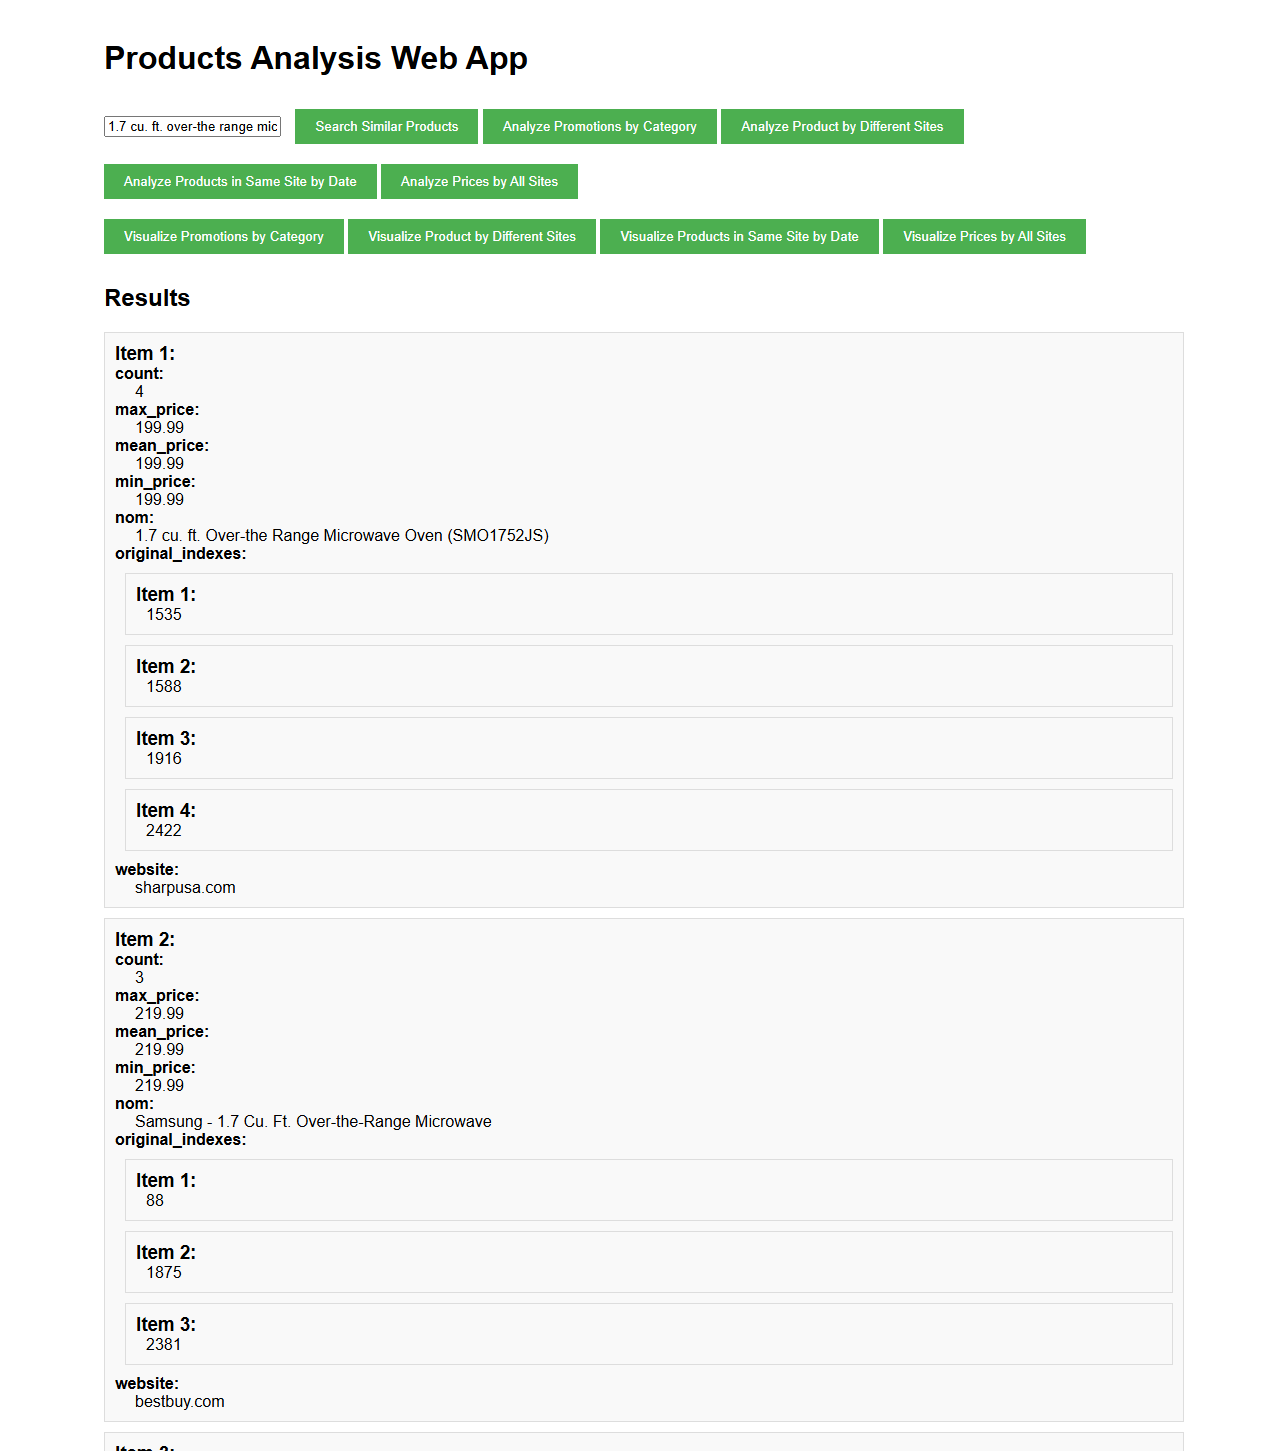
\includegraphics[width=1\linewidth]{fig/similar_products.png}
        \caption{Recherche de produit électroménager}
        \label{fig:similar_products}
    \end{figure}
    
    \item \textbf{Affichage des promotions :} L'interface offre également une section dédiée aux promotions. L'utilisateur peut naviguer à travers différentes catégories de produits électroménagers pour consulter les offres spéciales. L'API fournit la liste des promotions disponibles, qui est ensuite affichée sous forme de list.
    \begin{figure}
        \centering
        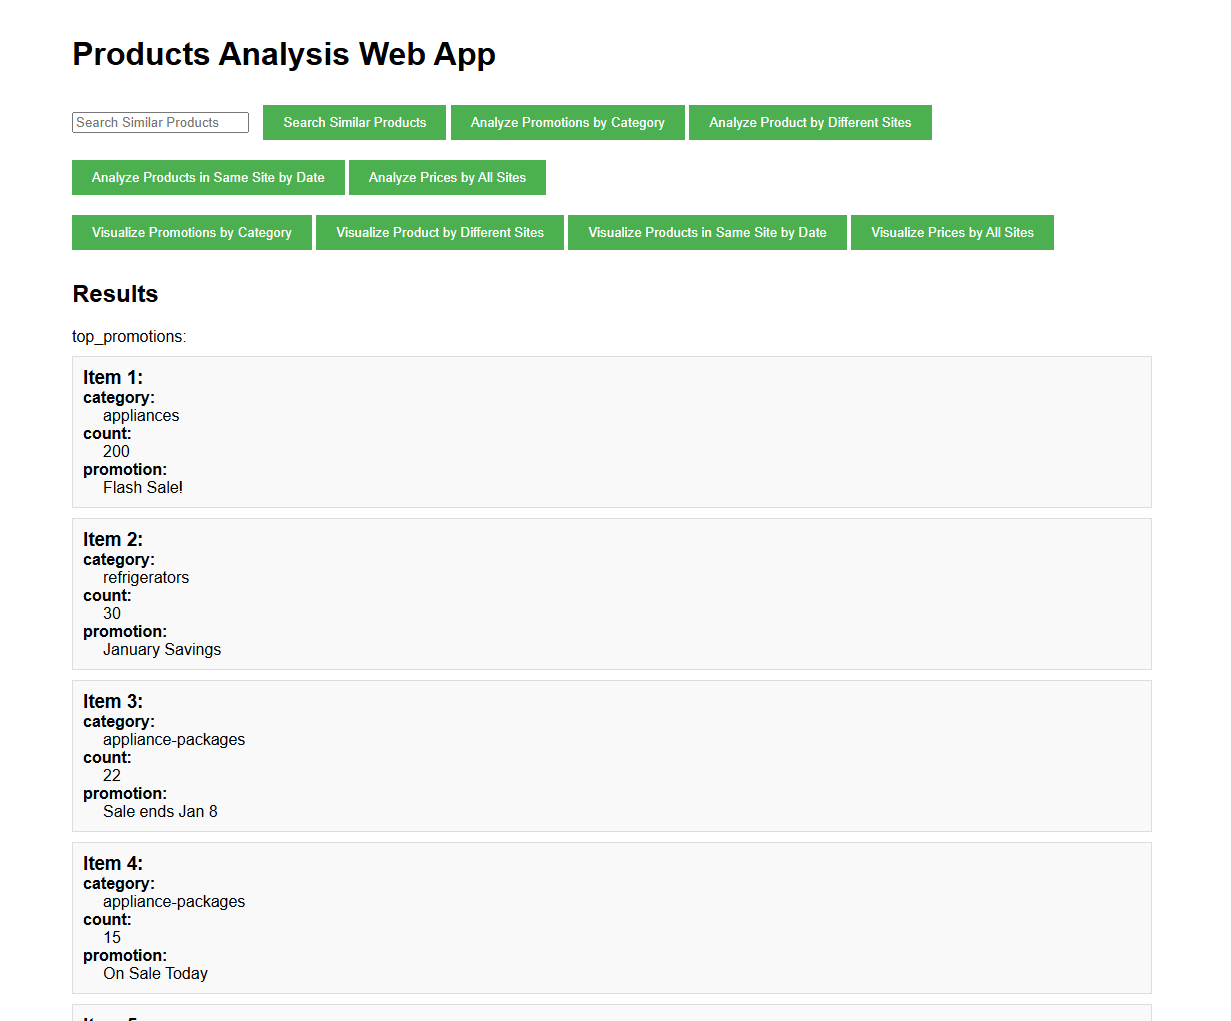
\includegraphics[width=1\linewidth]{fig/top_promotions.png}
        \caption{Affichage des promotions}
        \label{fig:promotions}
    \end{figure}
    
    \item \textbf{Affichage de prix entre plateformes :} Ce Affichage d'une graphique offre une vue claire des tendances des prix, permettant ainsi d'identifier les variations et d'assister dans la prise de décision stratégique pour l'achat de ce produit.
    \begin{figure}
        \centering
        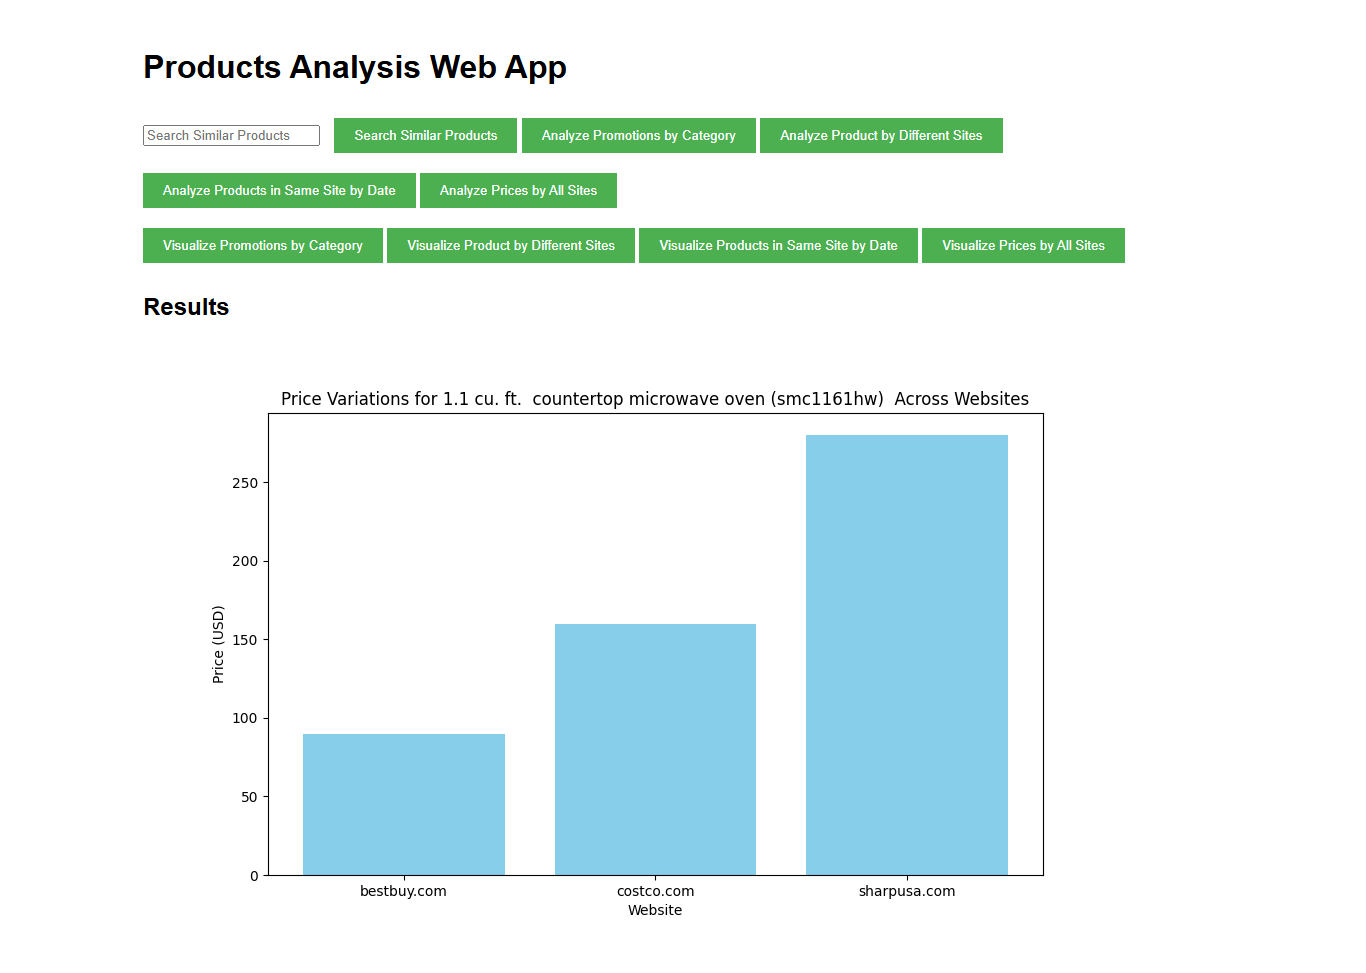
\includegraphics[width=1\linewidth]{fig/product_by_sites.png}
        \caption{Affichage de prix entre plateformes}
        \label{fig:plateformes}
    \end{figure}
    \item \textbf{Expérience utilisateur interactive :} Pour améliorer l'interaction, l'interface propose des éléments visuels comme des graphiques de comparaison des prix. Ces fonctionnalités sont alimentées par les données récupérées via l'API.
\end{itemize}

Cette interface rend l'accès aux résultats plus interactif et automatisé, permettant ainsi à l'utilisateur de bénéficier d'une expérience personnalisée et optimisée pour la recherche de produits et la consultation des offres.

\chapter{Difficultés Rencontrées}

Dans ce projet, plusieurs défis ont été rencontrés lors de l'extraction et de l'analyse des données des produits électroménagers. Ces difficultés ont nécessité des ajustements dans la méthodologie utilisée, ainsi qu'une gestion minutieuse des différents aspects du processus de collecte des données. Voici un aperçu des principales difficultés rencontrées.

\section{Problèmes liés au Web Scraping}

Outre les difficultés liées à l'extraction des caractéristiques des produits, des problèmes ont également surgi lors du processus de web scraping proprement dit. Ces difficultés incluent :

\begin{itemize}
    \item \textbf{Blocage des IP et captchas :} Plusieurs plateformes ont mis en place des mécanismes de sécurité pour empêcher le scraping de leurs sites. Des techniques comme les captchas ont été utilisées pour empêcher l'accès automatisé aux pages des produits. Pour contourner cela, des outils comme \texttt{Selenium} ont été utilisés avec des paramètres spécifiques pour simuler des actions humaines.
    \item \textbf{Limitations de la fréquence de scraping :} Certaines plateformes ont imposé des restrictions sur le nombre de requêtes pouvant être envoyées en une période donnée. Afin de ne pas surcharger les serveurs et éviter le blocage, des délais de pause ont été intégrés dans les scripts de scraping.
\end{itemize}

\section{Problèmes d'Extraction des Caractéristiques des Produits}

Une des difficultés majeures a été l'extraction des caractéristiques des produits, qui variaient fortement d'une plateforme à l'autre. Certains produits étaient décrits de manière très détaillée, tandis que d'autres avaient des informations plus limitées ou mal formatées. Cela a eu un impact sur la normalisation et la comparaison des données. Les problèmes rencontrés incluent :

\begin{itemize}
    \item \textbf{Descriptions incohérentes des produits :} Certaines plateformes utilisaient des termes différents pour décrire des produits similaires. Par exemple, un même modèle de réfrigérateur pouvait être nommé différemment selon le site. Il a donc été nécessaire d’harmoniser ces noms pour garantir la cohérence des données.
    \item \textbf{Caractéristiques manquantes ou incomplètes :} Plusieurs produits ne comportaient pas toutes les caractéristiques nécessaires pour une comparaison fiable (par exemple, la capacité du produit, les spécifications techniques). Cela a nécessité des techniques de recherche avancée ou même des estimations basées sur des informations similaires.
    \item \textbf{Variabilité des formats de présentation des caractéristiques :} Certaines plateformes présentaient les informations sous forme de tableaux, d’autres les affichaient sous forme de listes ou de paragraphes. Cette variabilité a créé des difficultés lors de l'extraction et de la structuration des données. Il a fallu adapter les scripts de scraping pour extraire correctement ces informations.
    \item \textbf{Caractères spéciaux et encodage :} Les pages des produits comportaient parfois des caractères spéciaux, ce qui compliquait l'extraction propre des informations. De plus, les différentes plateformes utilisaient divers encodages de caractères, nécessitant une normalisation et une conversion appropriée pour garantir l'intégrité des données.
\end{itemize}

\section{Conclusion sur les Difficultés Rencontrées}

Bien que ce projet ait rencontré plusieurs défis techniques, ceux-ci ont été surmontés grâce à l'utilisation de bibliothèques et de méthodologies adaptées. Le processus collecte des données a été particulièrement complexe, mais les solutions mises en place ont permis de garantir la qualité et la cohérence des informations utilisées pour l'analyse. Ces difficultés ont permis d'acquérir une expérience précieuse dans la gestion des données non structurées et le scraping web, tout en renforçant la compréhension des défis liés à l'analyse des données provenant de sources multiples et hétérogènes.


\chapter{Conclusion Générale}
Ce projet a permis d’explorer et d'analyser les variations des prix et des promotions des produits électroménagers sur plusieurs plateformes de commerce en ligne. L'objectif principal était de comprendre les tendances tarifaires et les stratégies de promotion utilisées dans le secteur de l’électroménager, en mettant l'accent sur les pratiques tarifaires et les effets des promotions sur le prix des produits.

L'analyse des prix a révélé des écarts significatifs entre les différentes plateformes, ce qui montre l'importance de comparer les offres pour obtenir le meilleur prix. Ces variations peuvent être influencées par plusieurs facteurs, tels que la saisonnalité, les politiques de prix des plateformes et les promotions temporaires. Le scraping des données a permis de collecter des informations actualisées et de garantir que l’analyse repose sur des données pertinentes et récentes.

L’identification des promotions a permis de mettre en lumière les stratégies de réduction de prix les plus courantes, telles que les ventes flash et les réductions saisonnières. Ces promotions ont un impact direct sur les décisions d’achat des consommateurs, en particulier pendant les périodes de vente importantes, comme les événements de début d'année.

Le nettoyage et la préparation des données ont également joué un rôle crucial dans la qualité des résultats. En éliminant les doublons et en harmonisant les noms des produits, nous avons pu garantir la fiabilité des informations analysées. L'utilisation d'outils comme Selenium, RapidFuzz et les threads a permis de rendre le processus de collecte des données plus rapide et plus efficace, tout en respectant les contraintes légales liées au web scraping.

En termes de visualisation, l’utilisation d’histogrammes et de diagrammes en barres a facilité la compréhension des résultats et a permis de visualiser les différences de prix et la fréquence des promotions par catégorie de produit. Ces graphiques ont non seulement permis d'identifier des tendances importantes, mais aussi de fournir une base solide pour des analyses futures.

\newpage

\section*{Perspectives}

Les résultats obtenus ouvrent la voie à plusieurs améliorations possibles et à de nouvelles explorations. Tout d'abord, l'intégration de données provenant d'autres sources, comme des avis clients ou des informations sur la qualité des produits, pourrait enrichir l'analyse et offrir une vue d'ensemble plus complète des facteurs influençant les décisions d'achat des consommateurs. De plus, la mise en place d'un modèle de prévision basé sur des techniques d'apprentissage automatique permettrait d'anticiper les évolutions des prix et des promotions.

Enfin, le processus de collecte de données pourrait être étendu à d'autres catégories de produits pour fournir une analyse encore plus détaillée des pratiques tarifaires dans le secteur du commerce en ligne. L'application de méthodes avancées de nettoyage des données et de gestion des informations massives (Big Data) pourrait améliorer la précision des analyses futures.

En conclusion, ce projet a fourni des insights précieux sur les stratégies tarifaires dans le domaine des produits électroménagers, tout en mettant en évidence l'importance de la collecte et du nettoyage des données dans l’analyse des tendances économiques. Les résultats obtenus peuvent aider les consommateurs à prendre des décisions d'achat éclairées et offrir aux plateformes de commerce en ligne des informations utiles pour optimiser leurs stratégies commerciales.

\newpage
\phantomsection
\addcontentsline{toc}{chapter}{Bibliographie}
\bibliography{References}  % référence à un fichier .bib
%\bibliographystyle{plain}
\bibliographystyle{unsrt}

\end{document}
